% !TeX root = ../main.tex
\chapter{Broadband photon pair generation}

Back to the classical nonlinear optics theory, the solution to nonlinear coupling equations requires at least the initial power at ether signal or idler mode, which is called seed in the laser terminology. However, in quantum classical theory, all the modes in cavity behave intrinsic vacuum fluctuation at the quantity of half $ \hbar \omega $. Thus, even without light fed, the quantum fluctuation leads to enhancement at the single photon levels. The intracavity pump power then behaves the amplifier, intensify the corresponding signal or idler mode photon flux. Once the single photon flux exceeds cavity threshold, the extracavity single photon can be detected. To note, these kind of excitation is indistinguishable because the signal and idler photons are emitted simultaneously as a result of quantum mechanics, rather than signal photon stimulates idler photon and vice versa. In the context of quantum states, the state created intracavity is at the superposition of signal state and idler state. The wave packet is different from the normal single photon one. Further theoretical research \cite{Scully1997} explained the squeezed nature of four wave mixing photon pairs, which is one of the exclusive properties of frequency entangled photon pair.

In general, the spontaneous four wave mixing in nonlinear cavities defined in our context refers to the cavity modes are excited collectively and pair-by-pair under the phase matching condition. Thus, under the weak coherent approximation, the photon pair only include one photon in each mode but correlated with each other. Thus, the conventional coincidence counting technology can be used to verify such correlation. In the term of generation band, it agrees with the classical phase matching condition at pump power limit.

%Furthermore, 
%To clarify with the physics compared with the relevant research, such as Kerr frequency comb and soliton generation, where ultra-high power is used to built intracavity pump mode, the spontaneous four wave mixing differs 
%\cite{Chembo2016a}

\section{Methods}

Using the dispersion extraction method in previous chapter, it is easy to locate zero dispersion wavelength among the telecom band. This range is preferred due to enormous available fiber optical components so that it is convenient to deploy totally in-line setups.
It is worth to mention that in our research, the main topic is generation rather than manipulation, so that numerous band-pass filter are exploited to realized mode-resolvable single photon counting. It does not contradict with the distinguishability of photon pair nature.

The setups 

\begin{figure}
	\centering
	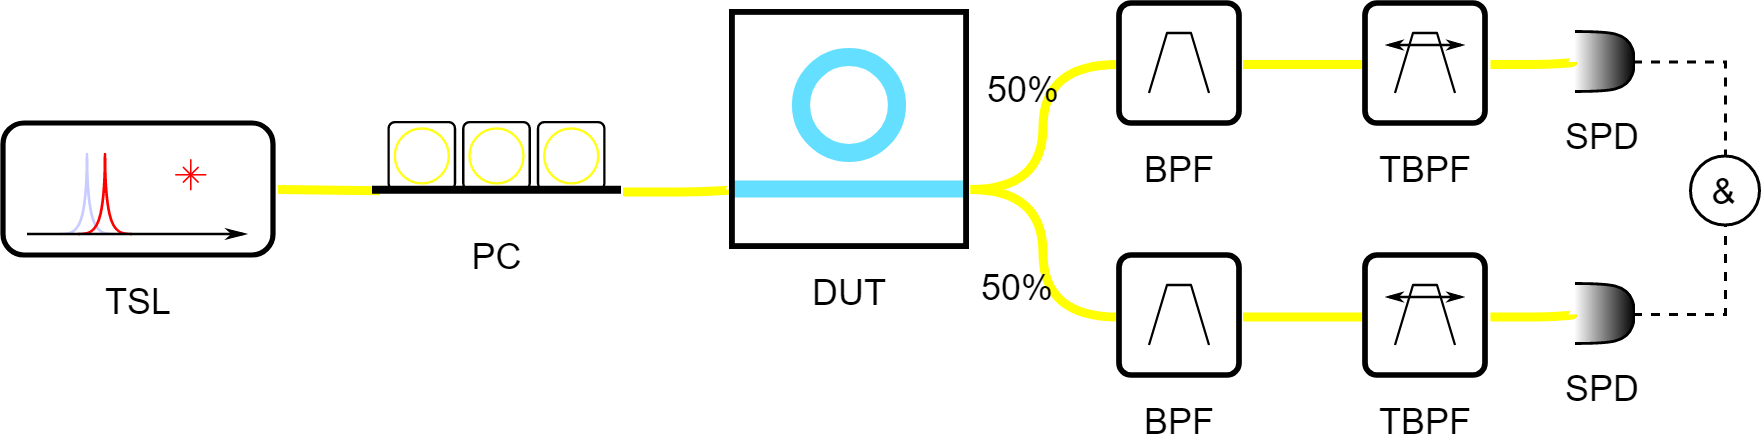
\includegraphics[width=0.7\linewidth]{imgs/png/biBPF}
	\caption{Mode-resolvable singular photon pair generation}
	\label{fig:bibpf}
\end{figure}



%The reason why optical telecom band is chosen in this research is that numerous fiber optical components are supplied in this range so that it is convenient to employ experiments requiring enormous optical components. In order to realize mode-resolvable photon pairs generation, 

\section{Coincidence counts}






\section{Coincidence counts vs. pump}

